\subsection {销售机会管理方法}

    销售机会管理有很多不同的名称,常用的名称有商机管理和销售漏斗管理,适用于大型复杂订单的销售,常用于直接销售和专卖店销售两种模式。

    96年,IBM在中国开始推行销售机会管理,现在已经形成了一套完整的体系,并且依赖这个体系来驱动销售目标的实现。

    每周一,销售人员将销售报表交给直接的主管,并在部门会议中逐一分析重要的销售机会,确定行动计划;周二,销售主管汇总自己的所有销售机会,与二线主管进行汇报,并讨论确定的销售计划;周三,二线主管与中国区的主管汇报和讨论销售机会和销售行动;周四,中国区的主管将汇总的报表交给亚太区的主管,取得他的认可;周五,全球的报表就到了全球总裁的桌面。IBM就是这样由下到上进行销售机会的管理。

    销售机会管理的本质是通用的公司用于管理销售机会的工具和方法。虽然不同的公司的称呼不一样,但跨国公司对于大型和复杂订单几乎都采用类似的工具。这种方法提供了销售团队关于进行沟通的语言,例如各个销售阶段的定义,并且提供了衡量销售机会和关键的过程性的指标。

    销售机会管理也体现了大型订单销售的精华,销售人员应该能够识别采购阶段,针对不同客户采取不同的销售策略。

    销售机会管理包括表格或者系统中的部分,也应该包括系统外的定期的销售会议,进行讨论、行动计划、反馈和总结。

\subsection {销售机会的分级}

    张学生以前是一家大公司的销售代表,他的太太就职于另外一家大型公司,他们在五年前买了一辆富康轿车。由于工作繁忙,没有时间学车,这部车一直由太太驾驶。

    一年前,他离开公司自己创业,开了一家印刷公司。由于需要经常在公司外与客户应酬,因此考了驾驶执照,开始开车。客户搭车的时候,富康安明显感觉到富康不能体现公司的形象,因为它与一家成功公司的总经理很不协调。因此希望换一部车。

    他的家里只有一个孩子,每个月的纯收入大约在两万元左右,因此他们商量后,决定购买一辆既能家用又能公司用的国产的中高档轿车。

    周末,他与太太常常去各个品牌的专卖店,已经看过雅阁、君威、奥迪和宝马。陆续排除了雅阁和君威,决定在奥迪和宝马中选择一辆。

    半年前,两人多次去看了宝马和奥迪的专卖店,张先生很喜欢奥迪A4,太太喜欢宝马325。由于担心汽车降价,因此两人决定持币观望,再等等。

    终于,听说奥迪开始于七月份做促销,可以得到额外的折扣,因此两人去专卖店查询。两人获知,除了折扣外,还可以额外得到大约一万元的折扣。

    两人去其它奥迪专卖店去进行了比较,包括价格,折扣和服务,最终选择了距离自己家和公司较近的专卖店。在专卖店的销售人员安排下,进行了试驾。

    之后,与销售代表进行谈判,确认了价格和赠送的配置。本来,两人还想再等等,但听说奥迪A4原装的CKD的产品只剩两台,以后就是SKD组装的,因此迅速将这台奥迪A4在国庆前买回家。

    没想到,十一刚过,就得到了奥迪降价的消息,这让他们很不满意,因此与奥迪专卖店交涉。在没有结果的情况下,他们非常不满意。最近,他的一位朋友也希望买奥迪,富康安坚决推荐他去另外一家专卖店购买。

    像案例中的客户一样,一家汽车销售公司有很多这样的销售机会,所有的订单都是从这些销售机会中产生的,如何管理这些销售机会呢?首先,我们要将案例中机会分成几个阶段。

\subsection {销售机会的管理指标}

    销售人员要识别客户的采购阶段,因为在不同阶段客户关心不同要点。对于向大型机构的采购,不同的客户在不同采购阶段起到主要的作用。

    \begin{center}
        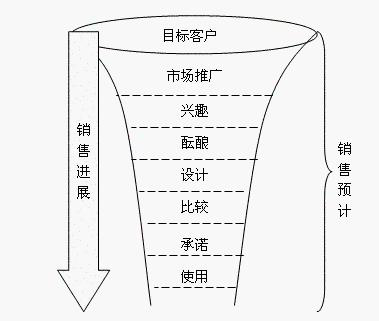
\includegraphics[scale=.6] {loudou1.png}
    \end{center}

    识别销售机会的阶段后就可以对销售机会进行管理了。我们可以将销售想象成一个漏斗,一些销售机会漏掉了,有一些销售机会经过采购流程的各个阶段转变成为订单。销售漏斗中有足够的销售机会并且不断地向下流动,转变成订单,直到达成销售目标。衡量销售机会是否足够的指标就是销售预计,衡量销售机会是否向下流动的指标就是销售进展。这两个量化的指标就是销售漏斗管理的核心的过程性指标。

    \begin{enumerate}
        \item 销售预计:

        销售团队或者成员中,处于各个采购阶段的销售机会的金额乘以这个阶段赢率的总和。销售机会可以用下面的计算公式表示:

        销售预计=∑(销售机会额X阶段赢率)

        每个销售人员必须有足够多的机会才可以完成任务,如果销售预计小于剩余的销售任务,那么销售人员就需要继续寻找销售机会。

        \item 销售进展:

        销售进展表示销售团队或者销售人员的销售机会转变成销售订单的速度。通常上市公司每个季度公布自己的财务数据,而销售管理又是以周进行。销售进展是根据每周的销售数字与季度的销售任务,计算后得到的。

        销售进展的计算方法是:本周销售预计加上本周累计销售额减去上周销售预计和上周累计销售额除以本季度的销售任务。由于一个季度有十三个周,因此销售人员每周的进展应该达到7.8%。

        \item 漏斗外销售额:

        对于为了使得销售漏斗管理简单易行,避免大量的录入工作,很多小型订单必须排除在销售漏斗以外。通常是以订单的金额为界限,低于一定金额的订单就不纳入销售漏斗管理。由于这个这个指标,销售预计和销售进展的计算公式要进行适当的修改。
    \end{enumerate}

    通过上述三个过程性指标就可以很好的管理销售多个机会,对每个目标客户分析需要更加深入的分析方法。
